\documentclass[12pt]{article}
\usepackage{graphicx}

\setlength{\textwidth}{6.5in}
\setlength{\oddsidemargin}{0.00in}    
\setlength{\topmargin}{0in}
\setlength{\headheight}{0in}
\addtolength{\textheight}{+1.0in}   

\def\Eq#1{Eq.~\ref{#1}} 
\def\Eqs#1#2{Eqs.~\ref{#1}--\ref{#2}} 
\def\Fig#1{Fig.~\ref{#1}} 

\def\Ca{${\rm Ca}^{2+}$}
\def\ca{[{\rm Ca}^{2+}]}
\def\ip{[{\rm IP}_{3}]}
\def\cae{[{\rm Ca}^{2+}]_{er}}
\def\Cai{$[{\rm Ca}^{2+}]_{i}$}
\def\Ip{${\rm IP}_{3}$}
\def\Ipr{${\rm IP}_{3}{\rm R}$}

\input{math_def}

\begin{document}             

\begin{center}
\section*{\boldmath An Example Latex File: \\
The Success of Whole Cell Models of \Ca\ Signaling}  
\end{center}

Regenerative \Ca\ release from the endoplasmic reticulum (ER), a continuous
membrane-delimited intracellular compartment, plays an important role in \Ca\
signaling\ \cite{Berridge93,Berridge97}.   
In most cell types the ER has integrative and regenerative
properties analogous to the excitable membranes of 
neurons\ \cite{Berridge98,LiEtal95a,KeizerEtal95}.  For example,
agonist-induced \Ca\ signaling in pituitary gonadotrophs is initiated by
metabotropic receptors of the plasma membrane that stimulate the production of
the intracellular messenger, inositol 1,4,5-trisphosphate (\Ip)
\cite{LiEtal94}.  \Ip\ in turn promotes \Ca\ release from intracellular stores
by binding and activating \Ipr\ receptor \Ca\ channels (\Ipr s) located on the
ER membrane.  In rat basophilic leukemia cells, an experimental model for
mucosal mast cells, cross-linking the high-affinity immunoglobulin E receptor
with multivalent antigen leads to tyrosine kinase-dependent 
activation of PLC$_\gamma$, production of \Ip, release of  
intracellular \Ca\ stores, and a sustained phase of \Ca\ influx---events 
that culminate in the secretion of histamine, serotonin,
and other mediators of inflammation\ \cite{WilsonEtal98,SmithEtal96}. 

\begin{figure}[h]
\centerline{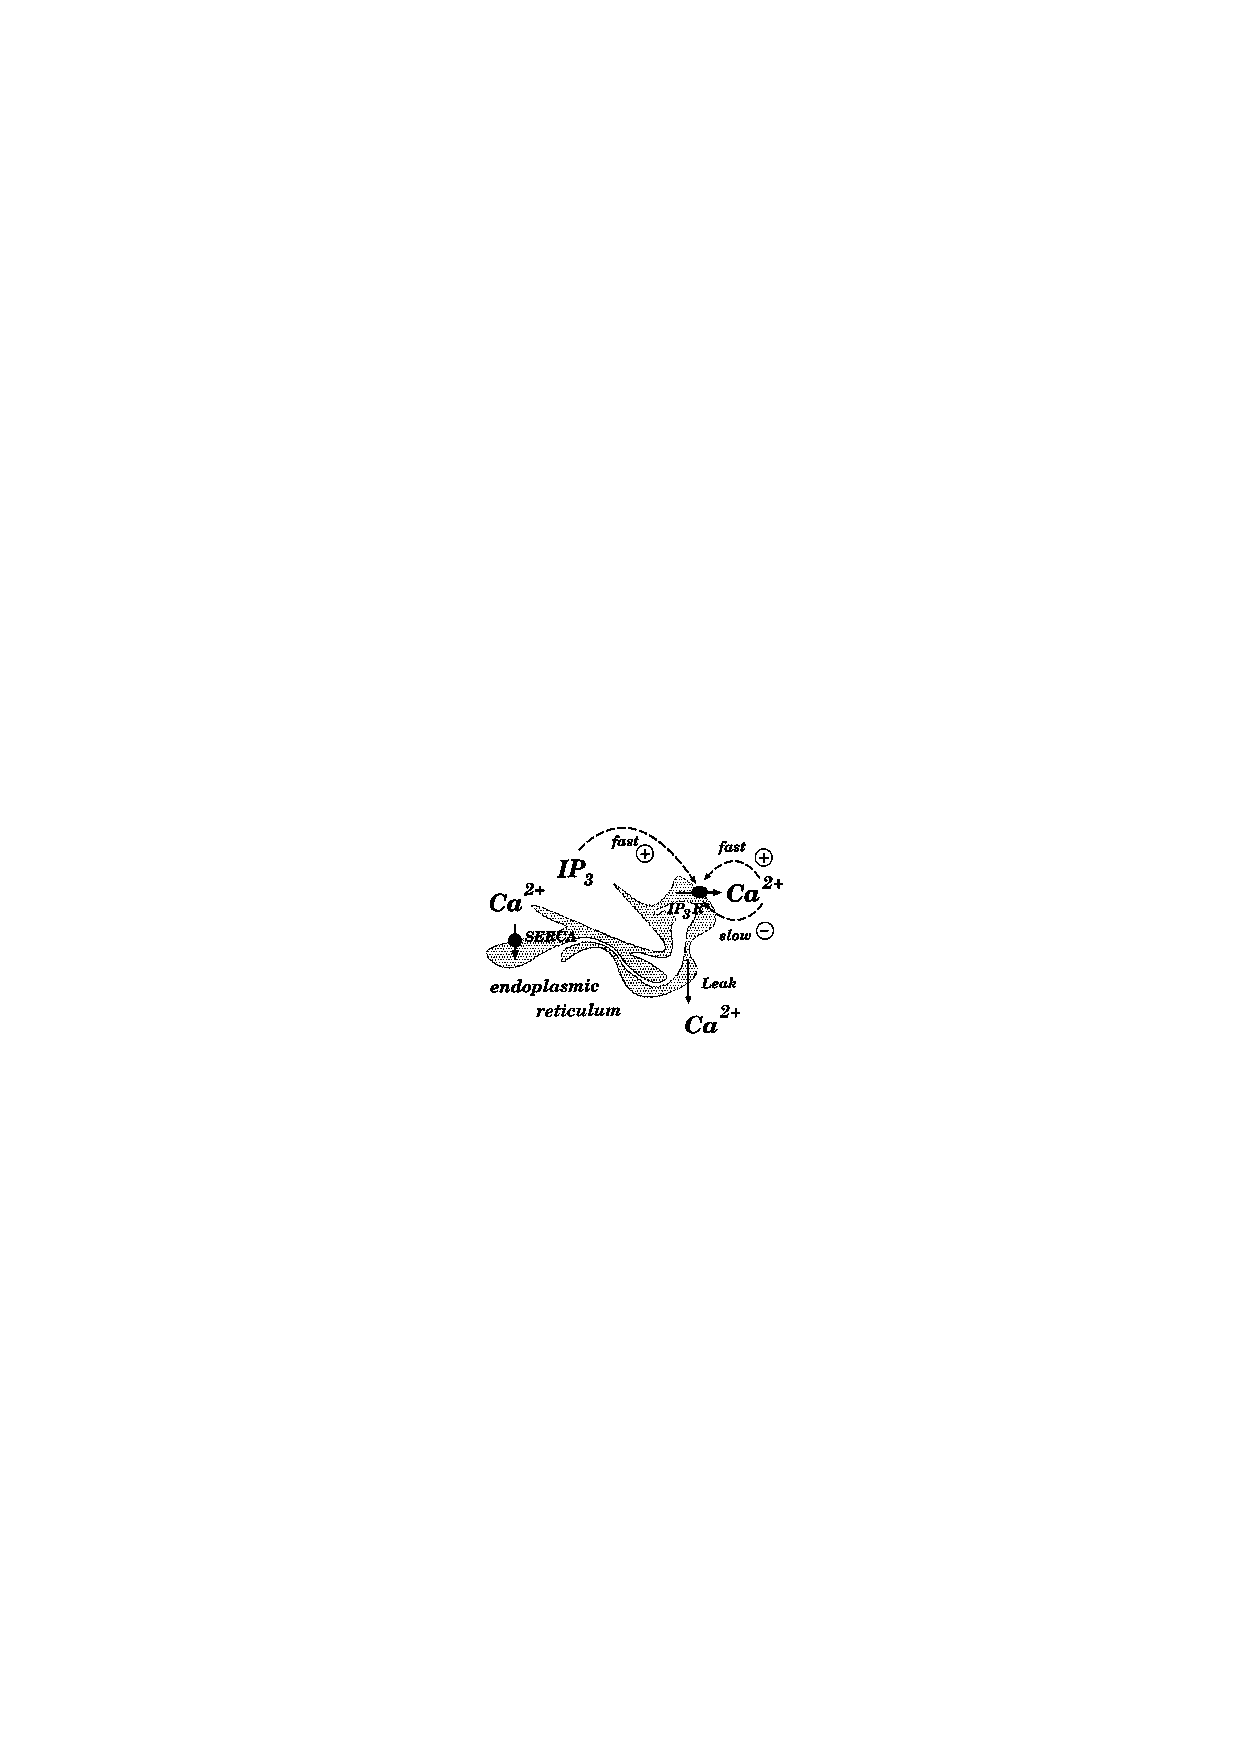
\includegraphics[height=2.0in,width=3.0in,angle=0]{FigureA.pdf}}
\caption{Schematic diagram of a whole cell model of \Ca\ handling. \Ca\ enters the
cytosol from the ER via a passive leak and the \Ipr, which is activated by
both \Ca\ and \Ip\ on a fast time scale and inhibited by \Ca\ on a slow time
scale, all at the cytoplasmic face.  The ER is refilled by a SERCA-type
\Ca-ATPase pump.  
Reproduced with permission from Jafri and Keizer, 1994.}
\label{FigureA}
\end{figure}

Whole cell models of intracellular \Ca\ signaling
have played a role in understanding the dynamics of \Ca\ responses
of gonadotrophs, RBL cells, and other cell types (reviewed 
in\ \cite{DuPontEtal91,DuPontGoldbeter92,LiEtal95a,KeizerEtal95}). 
While such models can be diagrammed as in Fig.~1, they are in
reality systems of nonlinear ODEs. For 
example, a whole cell model of \Ip-mediated \Ca\ responses
might take the following form,
\bne 
\ddt{\ca} = \underbrace{ j_{rel} - 
j_{up} }_{j_{er}} + \underbrace{j_{in} - j_{out}}_{j_{pm}} \quad\quad
\ddt{\cae} = -\alpha_{er} j_{er} \quad\quad
\label{WholeCellA}
\ene 
\bne 
\ddt{w} = \left[ w_\infty\left( \ca, \ip \right) - w \right] / \tau 
\left( \ca, \ip \right)  
\label{WODE}
\ene 
\bne j_{rel}= \left( v_{leak} + 
v_{ip} f_o \right) \left( \cae  - \ca \right)
\quad\quad j_{up}=\frac{ v_{p} \ca^2}{\ca^2 + k_{p}^2 } 
\label{WholeCellB}
\ene
In these equations, $w$ is a
Hodgkin-Huxley-like gating variable representing the fraction of \Ipr s {\it
not} inactivated and $f_o$, the open fraction (or open probability) 
of the \Ipr s, is a function of $w$, $\ca$, and $\ip$.  

Whole cell models of \Ca\ handling are biophysically realistic to the extent
that they include details of molecular mechanism.  For example, sigmoidal
kinetics of the SERCA-type \Ca-ATPase\ \cite{LyttonEtal92} have been used 
in \Eqs{WholeCellA}{WholeCellB} and the parameter $\alpha_{er}$ 
accounts for an ER/cytosol volume ratio of $\sim 1/6$. 
One of the keys to biophysical realism of whole cell models 
is the functional form for the open probability of 
the \Ipr\ and the equation for \Ipr\
kinetics. Indeed, when I present \Eq{WODE}, I have in mind 
the Li-Rinzel reduction of the DeYoung-Keizer model\
\cite{DeYoungKeizer92} in which the \Ipr\ is viewed as a collection of $n$
independent subunits, each of which has one binding site for \Ip\ and two
binding sites for \Ca\ \cite{DeYoungKeizer92}.  Thus, three processes
(\Ip-potentiation, \Ca-activation, and \Ca-inactivation) produce eight
possible states for each \Ipr\ subunit (see Fig.~3). 
With parameters chosen
to fit binding data and the `bell-shaped' steady-state open
probability curve of the \Ipr\ as a function of [\Ca] measured
in planar lipid bilayer experiments\ \cite{BezprozvannyEtal91}, whole cell
models of \Ca\ handling can exhibit \Ca\ oscillations for
superthreshold  [\Ip].

Li and Rinzel derived a simplified version of the DeYoung-Keizer model \Ipr\ by
noticing that the fast processes of \Ip-potentiation and \Ca-activation are
essentially at equilibrium with the slower process of \Ca-inactivation\
\cite{ParkerIvorra90,LiRinzel94}.  In this quasi-static limit, the functional
forms of $w_\infty \left( \ca, \ip \right)$ and $\tau \left( \ca, \ip \right)$ in
\Eq{WODE} are found and the fraction of open \Ipr s is given by $f_o =
m_\infty^n w^n$ where $m_{\infty}(\ca,\ip)$ is an instantaneously equilibrating
activation gating variable. 
 

\bibliographystyle{unsrt} 
\bibliography{ca,smith}

\end{document}




